% !TEX program = xelatex

%%%%%%%%%%%%%%%%%%%%%%%%%%%%%%%%%%%%%%%%%
% Thin Sectioned Essay
% LaTeX Template
% Version 1.0 (3/8/13)
%
% This template has been downloaded from:
% http://www.LaTeXTemplates.com
%
% Original Author:
% Nicolas Diaz (nsdiaz@uc.cl) with extensive modifications by:
% Vel (vel@latextemplates.com)
%
% License:
% CC BY-NC-SA 3.0 (http://creativecommons.org/licenses/by-nc-sa/3.0/)
%
%%%%%%%%%%%%%%%%%%%%%%%%%%%%%%%%%%%%%%%%%

%----------------------------------------------------------------------------------------
%	PACKAGES AND OTHER DOCUMENT CONFIGURATIONS
%----------------------------------------------------------------------------------------

\documentclass[a4paper, 11pt]{article} % Font size (can be 10pt, 11pt or 12pt) and paper size (remove a4paper for US letter paper)
\usepackage[table]{xcolor}
\usepackage{fontspec}
\definecolor{keycolor}{RGB}{172, 42, 42}
\definecolor{mbleu}{RGB}{64,96,127}
\definecolor{vimvert}{RGB}{46, 139, 87}
\usepackage{hyperref}
\usepackage{placeins} 
% \setmainfont{Avenir Next}
% \setsansfont{Avenir Next}

\usepackage{xeCJK}

\usepackage{geometry}
\geometry{left=2.54cm, top=2.54cm, right=2.54cm, bottom=2.54cm}
\usepackage{subcaption}
\usepackage{tikz}
\usetikzlibrary{tikzmark}
\usepackage{listings}
\usepackage{color}
\usepackage{forest}
\usepackage{float}
\usepackage{makecell}
\usepackage[binary-units]{siunitx}
\usepackage{enumitem}

\lstset{
basicstyle=\small,%
escapeinside=``,%
keywordstyle=\color{blue} \bfseries,% \underbar,%
identifierstyle={},%
commentstyle=\color{blue},%
stringstyle=\ttfamily,%
%labelstyle=\tiny,%
extendedchars=false,%
linewidth=\textwidth,%
numbers=left,%
numberstyle=\tiny \color{blue},%
frame=trbl%
}
 
\newcounter{code}
\lstnewenvironment{code}[3][C++]%
  {%
    \renewcommand\lstlistingname{代码}
    \lstset{% frame=tb,
    language=#1,
    caption=#2,
    label=#3
    }
  }{}

% \usepackage{fancyhdr}
% \usepackage{lastpage}
% \pagestyle{fancy}
% \fancyhf{}
% \fancyfoot[R]{第 \thepage 页,共 \pageref{LastPage} 页}
% % \fancyfoot[C]{\thepage/\pageref{LastPage}}
% \renewcommand{\headrulewidth}{0pt} 
% \renewcommand{\footrulewidth}{0.4pt} 
\renewcommand{\lstlistingname}{Code} % Listing->Code

% \usepackage[protrusion=true,expansion=true]{microtype} % Better typography
\usepackage{graphicx} % Required for including pictures
\usepackage{wrapfig} % Allows in-line images
\usepackage{newfloat}
\usepackage{amsmath}
\usepackage{multirow}

\usepackage{mathpazo} % Use the Palatino font
\usepackage[T1]{fontenc} % Required for accented characters
\linespread{1.2} % Change line spacing here, Palatino benefits from a slight increase by default
% \setlength{\parskip}{0.2em}

\usepackage{indentfirst}
\setlength{\parindent}{2em}

\makeatletter
\renewcommand\@biblabel[1]{\textbf{#1.}} % Change the square brackets for each bibliography item from '[1]' to '1.'
\renewcommand{\@listI}{\itemsep=0pt} % Reduce the space between items in the itemize and enumerate environments and the bibliography

\renewcommand{\maketitle}{ % Customize the title - do not edit title and author name here, see the TITLE block below
\begin{center} % Right align
{\LARGE\@title} % Increase the font size of the title

\large{\@subtitle}

\vspace{1em} % Some vertical space between the title and author name

{\large\@author} % Author name
% \\\@date % Date

% \vspace{1.5em} % Some vertical space between the author block and abstract
\end{center}
}

\renewcommand{\figurename}{图}
\renewcommand{\tablename}{表}

%----------------------------------------------------------------------------------------
%	TITLE
%----------------------------------------------------------------------------------------

\title{\textbf{操作系统实验项目}\\ % Title
} % Subtitle
\newcommand\@subtitle{实现系统调用}

\author{郑戈涵\quad 17338233\quad 931252924@qq.com} % Institution

\date{2020年5月3日} % Date


%----------------------------------------------------------------------------------------

\begin{document}

\maketitle % Print the title section

%----------------------------------------------------------------------------------------
%	ABSTRACT AND KEYWORDS
%----------------------------------------------------------------------------------------

\renewcommand{\abstractname}{摘要} % Uncomment to change the name of the abstract to something else

\begin{abstract}
  本次实验共完成三个任务:实现中断保护,完成软中断程序编写,生成自己的COM程序
\end{abstract}

% \hspace*{3,6mm}\texttt{Keywords:} lorem , ipsum , dolor , sit amet , lectus % Keywords

\vspace{1em} % Some vertical space between the abstract and first section

\setcounter{tocdepth}{2}
\renewcommand{\contentsname}{目录}
\tableofcontents

% \vspace{2em} % Some vertical space between the abstract and first section

\pagebreak

\section{实验目的}

% 问题、方法、实验目的、意义
\begin{enumerate}
  \item 学习掌握PC系统的软中断指令
  \item 掌握操作系统内核对用户提供服务的系统调用程序设计方法
  \item 掌握C语言的库设计方法
  \item 掌握用户程序请求系统服务的方法
\end{enumerate}


\section{实验要求}

\begin{enumerate}
  \item 了解PC系统的软中断指令的原理
  \item 掌握x86汇编语言软中断的响应处理编程方法
  \item 扩展实验四的的内核程序,增加输入输出服务的系统调用。
  \item C语言的库设计,实现putch()、getch()、printf()、scanf()等基本输入输出库过程。
\end{enumerate}

\section{实验内容}

% 输入、输出形式,使用的数据结构,算法的描述,算法正确性说明,算法分析,算法实现所需变量,没有代码
\subsection{编写用于中断处理的现场保护和现场恢复的汇编过程}

修改实验4的内核代码,先编写save()和restart()两个汇编过程,分别用于中断处理的现场保护和现场恢复,内核定义一个保护现场的数据结构,以后,处理程序的开头都调用save()保存中断现场,
处理完后都用restart()恢复中断现场。

\subsection{重写和扩展实验三的的内核程序}

内核增加int 20h、int 21h和int 22h软中断的处理程序,其中,int 20h用于用户程序结束是返回内核准备接受命令的状态;int 21h用于系统调用,并实现3-5个简单系统调用功能;
int22h功能未定,先实现为屏幕某处显示INT22H。

\subsection{实现部分基本输入输出库过程}

进行C语言的库设计,实现putch()、getch()、gets()、puts()、printf()、scanf()等基本输入输出库过程,汇编产生libs.obj。

\subsection{执行调用自己设计的库过程的程序}

利用自己设计的C库libs.obj,编写一个使用这些库函数的C语言用户程序,再编译,在与libs.obj一起链接,产生COM程序。增加内核命令执行这个程序。


\section{实验原理}
\subsection{中断}
所有计算机都提供允许其他模块(I/O、存储器)中断处理器正常处理过程的机制。
\paragraph{中断的分类}  \cite{ostextbook}
% Please add the following required packages to your document preamble:
% \usepackage[table,xcdraw]{xcolor}
% If you use beamer only pass "xcolor=table" option, i.e. \documentclass[xcolor=table]{beamer}
\begin{table}[]
  \caption{中断的分类}
  \label{tab:class-int}
  \begin{tabular}{ll}
    \rowcolor[HTML]{FFFFFF} 
    {\color[HTML]{333333} 程序中断}   & {\color[HTML]{333333} 在某些条件下由指令执行的结果产生,如算术溢出、除数为0、} \\
    \rowcolor[HTML]{FFFFFF} 
    {\color[HTML]{333333}}   & {\color[HTML]{333333} 试图执行一条非法机器指令及访问用户不允许的存储器位置} \\
    \rowcolor[HTML]{FFFFFF} 
    {\color[HTML]{333333} 时钟中断}   & {\color[HTML]{333333} 由处理器内部的计时器产生, 允许操作系统以一定的规律执行函数}                           \\
    \rowcolor[HTML]{FFFFFF} 
    {\color[HTML]{333333} l/0中断}  & {\color[HTML]{333333} 由I/O控制器产生, 用于发信号通知一个操作的正常完成或各种错误条件}                       \\
    \rowcolor[HTML]{F8F8F8} 
  {\color[HTML]{333333} 硬件失效中断} & {\color[HTML]{333333} 由诸如掉电或存储器奇偶校验错之类的故障产生}                                   
\end{tabular}
\end{table}

\subsection{中断术语} \cite{intprocess}
\begin{itemize}
  \item 按中断源进行分类:发出中断请求的设备称为中断源。按中断源的不同,中断可分为:
    \begin{itemize} 
    \item 内中断:即程序运行错误引起的中断
    \item 外中断:即由外部设备、接口卡引起的中断
    \item 软件中断:由写在程序中的语句引起的中断程序的执行,称为软件中断
    \end{itemize}
  \item 允许/禁止(开/关)中断: CPU通过指令限制某些设备发出中断请求,称为屏蔽中断。
  \item 从CPU要不要接收中断即能不能限制某些中断发生的角度 ,中断可分为
  \begin{itemize} 
    \item 可屏蔽中断 :可被CPU通过指令限制某些设备发出中断请求的中断
    \item 不可屏蔽中断:不允许屏蔽的中断如电源掉电
  \end{itemize}
  \item 中断允许触发器:在CPU内部设置一个中断允许触发器,只有该触发器置“1”,才允许中断;置“0”,不允许中断。
  \item 指令系统中,开中断指令,使中断触发器置“1”
  \item 关中断指令,使中断触发器置“0”
  \item 中断优先级:为了管理众多的中断请求,需要按每个(类)中断处理的急迫程度,对中断进行分级管理,称其为中断优先级。在有多个中断请求时,总是响应与处理优先级高的设备的中断请求。
  \item 中断嵌套:当CPU正在处理优先级较低的一个中断,又来了优先级更高的一个中断请求,则CPU先停止低优先级的中断处理过程,去响应优先级更高的中断请求,在优先级更高的中断处理完成之后,再继续处理低优先级的中断,这种情况称为中断嵌套。
\end{itemize}

\subsection{中断处理的过程}\cite{intprocess}
下面是保护模式中断处理的过程,实模式类似。
\begin{enumerate}
  \item 系统将所有的中断信号统一进行了编号(一共256个:0~255),这个号称为中断向量,具体哪个中断向量表示哪种中断有的是规定好的,也有的是在给定范围内自行设定的。  中断向量和中断服务程序的对应关系主要是由IDT(中断向量表)负责。操作系统在IDT中设置好各种中断向量对应的中断描述符(一共有三类中断门描述符:任务门、中断门和陷阱门),留待CPU查询使用。而IDT本身的位置是由idtr保存的,当然这个地址也是由OS填充的。
  中断服务程序具体负责处理中断(异常)的代码是由软件,也就是操作系统实现的,这部分代码属于操作系统内核代码。也就是说从CPU检测中断信号到加载中断服务程序以及从中断服务程序中恢复执行被暂停的程序,这个流程基本上是硬件确定下来的,而具体的中断向量和服务程序的对应关系设置和中断服务程序的内容是由操作系统确定的。
  
  \item CPU在执行完当前程序的每一条指令后,都会去确认在执行刚才的指令过程中中断控制器(如:8259A)是否发送中断请求过来,如果有那么CPU就会在相应的时钟脉冲到来时从总线上读取中断请求对应的中断向量[2]。
  对于异常和系统调用那样的软中断,因为中断向量是直接给出的,所以和通过IRQ(中断请求)线发送的硬件中断请求不同,不会再专门去取其对应的中断向量。
  
  \item 根据中断向量到IDT表中取得处理这个向量的中断程序的段选择符
  CPU根据得到的中断向量到IDT表里找到该向量对应的中断描述符,中断描述符里保存着中断服务程序的段选择符。
  
  \item 根据取得的段选择符到GDT中找相应的段描述符
  CPU使用IDT查到的中断服务程序的段选择符从GDT中取得相应的段描述符,段描述符里保存了中断服务程序的段基址和属性信息,此时CPU就得到了中断服务程序的起始地址。这里,CPU会根据当前cs寄存器里的CPL和GDT的段描述符的DPL,以确保中断服务程序是高于当前程序的,如果这次中断是编程异常(如:int 80h系统调用),那么还要检查CPL和IDT表中中断描述符的DPL,以保证当前程序有权限使用中断服务程序,这可以避免用户应用程序访问特殊的陷阱门和中断门。
  
  \item CPU根据特权级的判断设定即将运行的中断服务程序要使用的栈的地址
  CPU会根据CPL和中断服务程序段描述符的DPL信息确认是否发生了特权级的转换,比如当前程序正运行在用户态,而中断程序是运行在内核态的,则意味着发生了特权级的转换,这时CPU会从当前程序的TSS信息(该信息在内存中的首地址存在TR寄存器中)里取得该程序的内核栈地址,即包括ss和esp的值,并立即将系统当前使用的栈切换成新的栈。这个栈就是即将运行的中断服务程序要使用的栈。紧接着就将当前程序使用的ss,esp压到新栈中保存起来。也就说比如当前在某个函数中,使用的栈,在中断发生时,需要切换新的栈。
  
  \item 保护当前程序的现场,CPU开始利用栈保护被暂停执行的程序的现场:依次压入当前程序使用的eflags,cs,eip,errorCode(如果是有错误码的异常)信息。
  \item 跳转到中断服务程序的第一条指令开始执行
  CPU利用中断服务程序的段描述符将其第一条指令的地址加载到cs和eip寄存器中,开始执行中断服务程序。这意味着先前的程序被暂停执行,中断服务程序正式开始工作。
  
  \item 中断服务程序处理完毕,恢复执行先前中断的程序
  在每个中断服务程序的最后,必须有中断完成返回先前程序的指令,这就是iret(或iretd)。程序执行这条返回指令时,会从栈里弹出先前保存的被暂停程序的现场信息,即eflags,cs,eip重新开始执行。
\end{enumerate}



\section{实验过程}

本次实验流程如下
\begin{enumerate}
  \item 编写中断向量操作程序
  \item 编写x86汇编语言对时钟中断的响应处理程序
  \item 编写对键盘中断的响应处理程序
  \item 修改内核和用户程序
  \item 生成镜像,在虚拟机中加载
\end{enumerate}

\subsection{编写中断向量操作程序}

\subsubsection{移动中断向量宏}
原则上虽然我们将要利用中断向量表来执行自己写的程序,但是被覆盖的中断的原本的功能应该还是有,因此需要将中断向量转移到其他的向量号上。
为了多次使用这段代码,我将其设为宏,代码如下:
\begin{lstlisting}[language={[x86masm]Assembler},label=MOVE VECTOR,caption=MOVE\_VECTOR]
  %macro MOVE_VECTOR 2
  pusha            ; 保护现场
  push es
  mov ax, 0
  mov	es, ax       ; 数据段
  mov ax, word[es:%1*4]
  mov word[es:%2*4],ax
  mov ax, word[es:%1*4+2]
  mov word[es:%2*4+2],ax
  pop es
  popa             ; 恢复现场
%endmacro
\end{lstlisting}
将 $ 0+\text{中断号}\times 4 $ 的位置的数据取出来放到目标中断号对应的位置即可



\subsubsection{中断向量写入宏}
写入中断向量也会多次用到,因此我将其设为宏,代码如下
\begin{lstlisting}[language={[x86masm]Ass
embler},label=VECTOR IN,caption=VECTOR\_IN]
  %macro VECTOR_IN 2
  pusha            ; 保护现场
  push es
  mov ax, 0
  mov	es, ax       ; 数据段
  mov word[es:%1*4],%2
  mov ax, cs
  mov word[es:%1*4+2],ax
  pop es
  popa             ; 恢复现场
%endmacro
\end{lstlisting}
将自己送入的中断程序的地址放入0开始中断号*4的偏移量的位置即可,注意每次放入的单位为一个字(word),第一个字为IP,第二个为CS。

\subsection{时钟中断的响应处理程序}
单个程序是作为引导程序的,因此尽量不能超过512字节,并且末尾两个字节为0x55aa。代码由老师提供的修改得到。代码如下:
\begin{lstlisting}[language={[x86masm]Assembler},label=TimerTest,caption=Timer(test)]
org 7c00h
%include "header.inc"
VECTOR_IN 08h,Timer
sti
jmp $			; 死循环
; 时钟中断处理程序

Timer:
    pusha
    push gs
    push ds
    mov ax,cs
    mov ds,ax
    mov	ax,0B800h		; 文本窗口显存起始地址
    mov	gs,ax		; GS = B800h

    dec byte [count]		; 递减计数变量
    jnz Exit			; >0:跳转
    mov byte[count],delay		; 重置计数变量=初值delay 
    mov ah,[color]
    dec byte[color]
    jz restoreColor
draw:
    mov si, wheel
    add si, [wheelOffset]
    mov al,[si]
  mov [gs:((80*24+79)*2)],ax	; =0:递增显示字符的ASCII码值
    inc byte[wheelOffset]
    cmp byte[wheelOffset],4
    jne Exit
    mov byte[wheelOffset],0
Exit:
    mov al,20h			; AL = EOI
    out 20h,al			; 发送EOI到主8259A
    out 0A0h,al			; 发送EOI到从8259A
    pop ds
    pop gs
    popa
    iret			; 从中断返回
%endmacro
\end{lstlisting}

\paragraph{主模块}
首先在第一行用org 0x7c00,这样可以不修改段基址而能正常读取内存中的数据,然后使用include将上面两节完成的代码引用进来,其中包括写入中断向量和移动中断向量的宏,由于测试时我同时使用了bochs,
而bochs执行引导程序时是会显示一段文字的,因此我选择在程序开始时清屏。设置好各个段的基址(gs=0B800h)然后将中断响应处理程序Timer所在的地址写入向量表,
然后最重要的一点是要开中断,否则时钟不会触发。

\paragraph{风火轮模块}
要实现风火轮,只要在显存里的某个位置轮流放入那四个字符即可,因此把他们按顺序放在内存中,然后用循环遍历他们即可,为了让风火轮显示不那么快,
我在每次显示之前都执行一段延迟的指令,然后进入绘制部分。绘制部分只需要用内存中的一个变量记住当前风火轮的位置,然后用寄存器将这个偏移量加到风火轮字符串对应的地址上,
得到需要的字符的地址,然后把字符放入显存里。我的程序每次还会改变风火轮的颜色,只要维护一个颜色的变量,每次写入显存前赋值到ah寄存器里即可。
每一次中断处理结束,需要发送一个EOI给8259A, 以便继续接收中断。最后iret返回。

修改一下上次的makefile,直接用make命令生成镜像即可。在vmware或bochs中打开。效果如下:

\begin{figure}[H]
  \centering
  
\includegraphics[width=0.8\linewidth]{mixtest.png}
  \caption{风火轮程序运行过程截图}
  \label{fig:mixtest}
\end{figure}

\subsection{键盘中断的响应处理程序}
键盘中断号为09h,处理程序只需要打印信息,然后返回即可。代码如下:

\begin{lstlisting}[language={[x86masm]Assembler},label=ouch.asm,caption=ouch.asm]
  %include "utility.inc"

  Ouch:
      pusha
      push ds
      mov ax,cs
      mov ds,ax
    PRINT msg, msg_len, 20, 40
      call Delay
    PRINT clearMsg, msg_len, 20, 40
      
      int 40h
  
      mov al,20h           ; AL = EOI
      out 20h,al           ; 发送EOI到主8529A
      out 0A0h,al          ; 发送EOI到从8529A
  
      pop ds
      popa
      iret
  msg db 'OUCH! OUCH!'
  msg_len equ $-msg
  clearMsg db '           '
  
  Delay:
      pusha
      mov ax,500
  dd:
      mov cx,50000
  ddd:
      loop ddd
      dec ax
      cmp ax,0
      jne dd
      popa
      ret
  
\end{lstlisting}
utility库中的函数是上一节中定义的写入向量等宏。由于该程序需要在用户程序中被执行,因此不能调用清屏,需要用空字符串来覆盖。在内存中定义好对应的字符串,
然后调用PRINT打印Ouch字符串,延迟一段时间,再打印空白字符串覆盖,然后发送EOI到8259A再iret返回即可。Delay方法和第一次实验一样。

\subsection{修改内核和用户程序}

时钟中断在内核运行时就需要,因此在内核初始化阶段应该将其地址送入中断向量表。键盘响应只需要在用户程序中运行,因此修改用户程序即可。

\subsubsection{修改内核}

为了让原来的时钟中断向量还能被使用,我将其放入0x39中,在内核开始时移动中断向量并将自己编写的程序的地址写入向量表即可。代码只有两句:
\begin{lstlisting}[language={[x86masm]Assembler},label=kernelChange,caption=内核程序更改]
  MOVE_VECTOR 08h,39H
  VECTOR_IN 08h,Timer
\end{lstlisting}
\subsubsection{修改用户程序}

和内核一样,键盘中断程序也需要移位,这次我放入0x40中,在用户程序开始时需要移动中断向量并将自己编写的程序的地址写入向量表,离开时需要恢复。
中断程序需要放在用户程序结尾。

\begin{lstlisting}[language={[x86masm]Assembler},label=userChange,caption=用户程序更改]
MOVE_VECTOR 09h,40h
VECTOR_IN 09h,Ouch
MOVE_VECTOR 40h,09h
%include "ouch.asm"
\end{lstlisting}

\subsection{扩展内核程序-实时显示时间}
由于上一次实验中内核已经比较完善,这次实验使用时钟中断为shell提供新的特性-显示时间,和实现风火轮一样,只要将对应的程序放入中断向量表中即可。
所以完成扩展总共有三个步骤:
\begin{enumerate}
  \item 从BIOS获得日期时间的信息
  \item 用c代码完成信息的加工和显示
  \item 修改中断程序
  \item 在合适的位置加载中断向量
\end{enumerate}

\subsubsection{从BIOS获得日期时间的信息}
从BIOS获得日期时间的信息是通过读端口实现的,首先设置好对应的寄存器,用寄存器向70h端口写入要访问的单元地址,然后从71h端口读入即可获得数据。
该函数是用来给c代码调用的,因此首先需要确定他的声明。为了使函数能够复用,可以把读端口需要设置的寄存器值作为参数传给汇编过程,
,为了代码的可读性,我为参数设计了枚举类型Date,总共有6项,请看表\ref{tab:enum-date}
\FloatBarrier



% Please add the following required packages to your document preamble:
% \usepackage[table,xcdraw]{xcolor}
% If you use beamer only pass "xcolor=table" option, i.e. \documentclass[xcolor=table]{beamer}
\begin{table}[]
\centering
\caption{日期时间枚举表}
\label{tab:enum-date}
\begin{tabular}{lll}
  名称 & 枚举变量名                                                          & 数值                                                        \\
  秒  & \cellcolor[HTML]{FFFFFF}{\color[HTML]{333333} \textbf{Second}} & \cellcolor[HTML]{FFFFFF}{\color[HTML]{333333} \textbf{0}} \\
  分  & \cellcolor[HTML]{FFFFFF}{\color[HTML]{333333} \textbf{Minute}} & \cellcolor[HTML]{FFFFFF}{\color[HTML]{333333} \textbf{2}} \\
  小时 & \cellcolor[HTML]{FFFFFF}{\color[HTML]{333333} \textbf{Hour}}   & \cellcolor[HTML]{FFFFFF}{\color[HTML]{333333} \textbf{4}} \\
  日  & \cellcolor[HTML]{F8F8F8}{\color[HTML]{333333} \textbf{Day}}    & \cellcolor[HTML]{F8F8F8}{\color[HTML]{333333} \textbf{7}} \\
  月  & Month                                                          & 8                                                         \\
  年  & Year                                                           & 9                                                        
\end{tabular}
\end{table}

函数的返回值是BIOS返回的数字,这些数字是BCD码,需要转换为十进制整数。

\subsubsection{加工和显示获得的信息}
要调用汇编的函数,首先需要用extern声明该函数。获得日期时间对应的数字信息后,利用上次实验实现的数字转字符串函数就能得到对应的字符串,然后加工需要用到strcat函数,
合成成一个完整的字符串就可以显示了.为了美观,显示小于10的数字前我都手动补了0,保证不会总是跳动。工具函数的代码请看附录的\ref{utilsForDisp},显示的c代码如下:
\begin{lstlisting}[language={c},label=split,caption=split]
  void printDate(){
    int year=getDateInfo(Year),
    month=getDateInfo(Month),
    day=getDateInfo(Day),
    hour=getDateInfo(Hour),
    minute=getDateInfo(Minute),
    second=getDateInfo(Second);

    char TimeBuffer[22]={0};
    char *yearPrefix = "20";
    strcat(TimeBuffer, yearPrefix);
    strcat(TimeBuffer, itoa(bcd2dec(year), 10));
    strAppend(TimeBuffer, '-');
    if(month<10){
        strAppend(TimeBuffer, '0');
    }
    strcat(TimeBuffer, itoa(bcd2dec(month), 10));
    strAppend(TimeBuffer, '-');
    if(day<10){
        strAppend(TimeBuffer, '0');
    }
    strcat(TimeBuffer, itoa(bcd2dec(day), 10));
    strAppend(TimeBuffer, ' ');
    if(hour<10){
        strAppend(TimeBuffer, '0');
    }
    strcat(TimeBuffer, itoa(bcd2dec(hour), 10));
    strAppend(TimeBuffer, ':');
    if(minute<10){
        strAppend(TimeBuffer, '0');
    }
    strcat(TimeBuffer, itoa(bcd2dec(minute), 10));
    strAppend(TimeBuffer, ':');
    if(second<10){
        strAppend(TimeBuffer, '0');
    }
    strcat(TimeBuffer, itoa(bcd2dec(second), 10));

    printPos(TimeBuffer,20,24,58);
}
\end{lstlisting}
其中使用的printpos和itoa都是上次实验实现的。限于篇幅,代码不在此放出。注意,之前使用的printpos函数是参考的老师的代码,老师的版本会移动光标,使用这个版本会导致光标永远集中在显示的时间字符串后面,
无法输入shell命令,因此在调用10号中断前需要设置al=0而非1(将光标置于串尾)。

\subsubsection{修改中断程序}
由于显示时间会挡住用户程序的显示,而且由于两者可能会同时修改显存,有时候会产生问题,所以我设置了两份中断程序,一份用于内核,带时间和风火轮,一份用于用户程序,只有风火轮。只用风火轮的不需要修改,
用户程序的只需要在返回前调用显示日期时间的c函数即可。

\subsubsection{在合适的位置加载中断向量}
\paragraph{修改内核程序}
由于要安排两个版本,内核程序和加载用户程序的函数都需要修改,在5.4.1小节的基础上,内核程序只需要修改放入的地址为新中断程序的地址即可。

\paragraph{修改加载用户程序的函数}
加载用户程序前需要将只有风火轮的中断程序地址放入中断向量表,从用户程序返回后再将新的中断程序地址放入向量表。

\subsection{软盘扇区安排}

由于修改的内容都是在原有代码的基础上修改的,没有增加新的程序,所以扇区安排和上次一样,安排请看表\ref{tab:sectortable}:
\FloatBarrier
% Please add the following required packages to your document preamble:
% \usepackage[table,xcdraw]{xcolor}
% If you use beamer only pass "xcolor=table" option, i.e. \documentclass[xcolor=table]{beamer}
\begin{table}[]
\centering
  \caption{软盘扇区安排}
  \label{tab:sectortable}
  \begin{tabular}{llll}
  \rowcolor[HTML]{FFFFFF} 
  {\color[HTML]{333333} \textbf{磁头号}} & {\color[HTML]{333333} \textbf{扇区号}} & {\color[HTML]{333333} \textbf{扇区数(大小)}} & {\color[HTML]{333333} \textbf{内容}} \\
  \rowcolor[HTML]{FFFFFF} 
  {\color[HTML]{333333} 0}            & {\color[HTML]{333333} 1}            & {\color[HTML]{333333} 1(512 B)}         & {\color[HTML]{333333} 引导程序}        \\
  \rowcolor[HTML]{FFFFFF} 
  {\color[HTML]{333333} 0}            & {\color[HTML]{333333} 2$\sim$17}    & {\color[HTML]{333333} 16(8 KB)}         & {\color[HTML]{333333} 操作系统内核}      \\
  \rowcolor[HTML]{F8F8F8} 
  {\color[HTML]{333333} 1}            & {\color[HTML]{333333} 1$\sim$2}     & {\color[HTML]{333333} 2(1 KB)}          & {\color[HTML]{333333} 用户程序1(LU.com)}       \\
  \rowcolor[HTML]{FFFFFF} 
  {\color[HTML]{333333} 1}            & {\color[HTML]{333333} 3$\sim$4}     & {\color[HTML]{333333} 2(1 KB)}          & {\color[HTML]{333333} 用户程序2(LD.com)}       \\
  \rowcolor[HTML]{F8F8F8} 
  {\color[HTML]{333333} 1}            & {\color[HTML]{333333} 5$\sim$6}     & {\color[HTML]{333333} 2(1 KB)}          & {\color[HTML]{333333} 用户程序3(RU.com)}       \\
  \rowcolor[HTML]{FFFFFF} 
  {\color[HTML]{333333} 1}            & {\color[HTML]{333333} 7$\sim$8}     & {\color[HTML]{333333} 2(1 KB)}          & {\color[HTML]{333333} 用户程序4(RD.com)}      
  \end{tabular}
  \end{table}
\subsection{镜像文件生成}


使用gcc生成c源文件对应的汇编,nasm生成内核汇编源文件和库过程汇编源文件的elf格式的汇编,使用ld链接可以生成二进制文件,
将引导程序,内核程序和用户程序放入镜像中的合适位置即可生成镜像。

代码相关信息请看readme.md。

在wsl或linux的shell中执行\textit{make all/make img}即可生成镜像(.img)文件,在VMware中加载该镜像,查看结果。到此,实验结束。

\section{程序使用说明}
\subsection{实验环境}
\begin{enumerate}
  \item 调试,运行工具:bochs
  \item 汇编器:nasm 2.13.02
  \item 编译器:gcc 7.5.0
  \item 链接器:ld 2.30
  \item 编译环境:wsl Ubuntu
  \item VSCode 1.44.2
\end{enumerate}
% 如何编译和使用程序

\subsection{编译方法}

\subsubsection{系统要求}

生成镜像文件时,可以使用linux操作系统或者带wsl的windows系统。

\subsubsection{编译过程与参数}

在源代码目录下使用wsl,执行下列代码即可得到镜像文件os17338233.img。
\begin{code}{生成镜像}{code:generateos}
make
\end{code}

\subsection{运行与演示}

运行镜像时请使用bochs,如果使用vmware,在运行用户程序时会遇到问题,其他正常,bochs上是完全正常的。
\subsubsection{风火轮}
图 \ref{fig:sheel}是5.4节完成后的shell的界面
\begin{figure}[H]
  \centering
  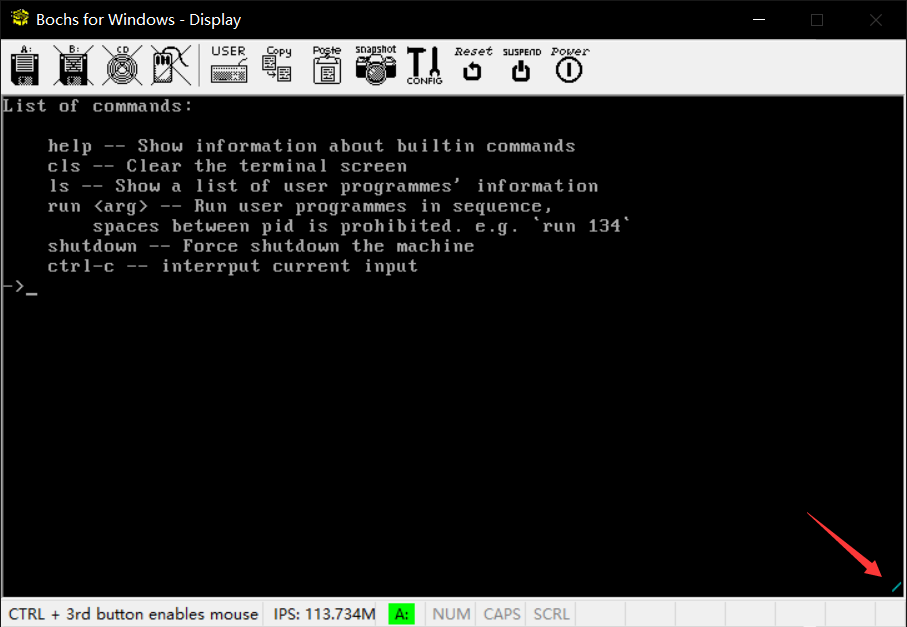
\includegraphics[width=0.8\linewidth]{shell.png}
  \caption{带风火轮的shell}
  \label{fig:sheel}
\end{figure}


\subsubsection{带时间显示和风火轮}

图\ref{fig:wheelentr}是5.5节完成后进入shell前的界面
\begin{figure}[H]
  \centering
  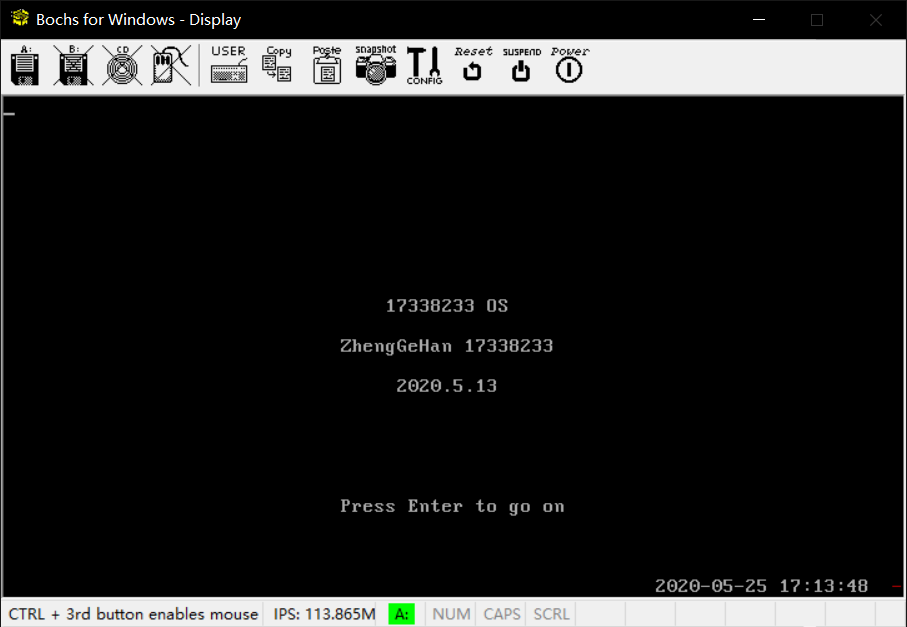
\includegraphics[width=0.8\linewidth]{entrWithDate.png}
  \caption{带时间显示和风火轮的shell进入界面}
  \label{fig:wheelentr}
\end{figure}

图\ref{fig:wheelShell}是5.5节完成后的shell的界面
\begin{figure}[H]
  \centering
  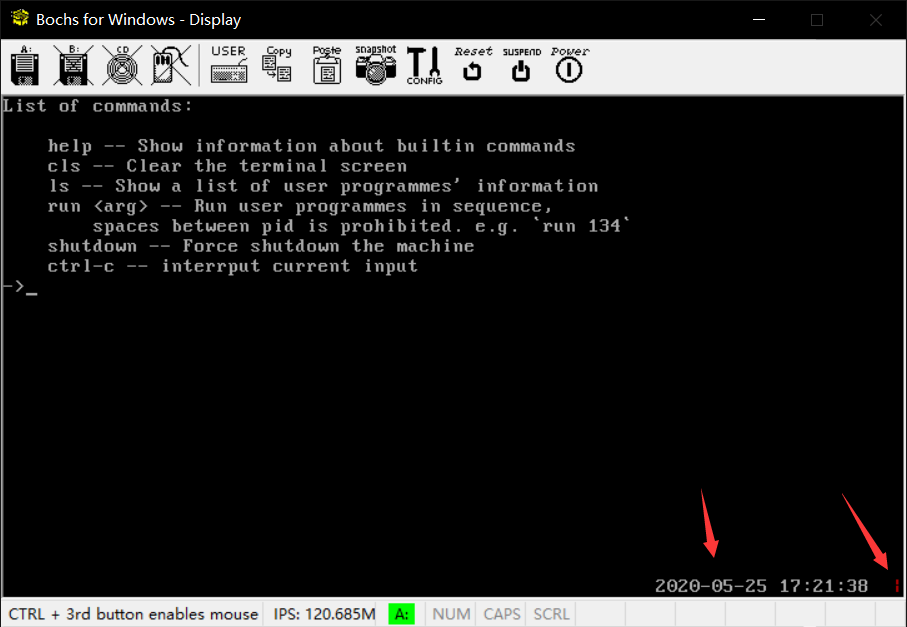
\includegraphics[width=0.8\linewidth]{shellWithDate.png}
  \caption{带时间显示和风火轮的shell}
  \label{fig:wheelShell}
\end{figure}



\subsubsection{带时间显示和风火轮}
进入用户程序后的效果如图 \ref{fig:timeDisp} 所示。
\begin{figure}[H]
  \centering
  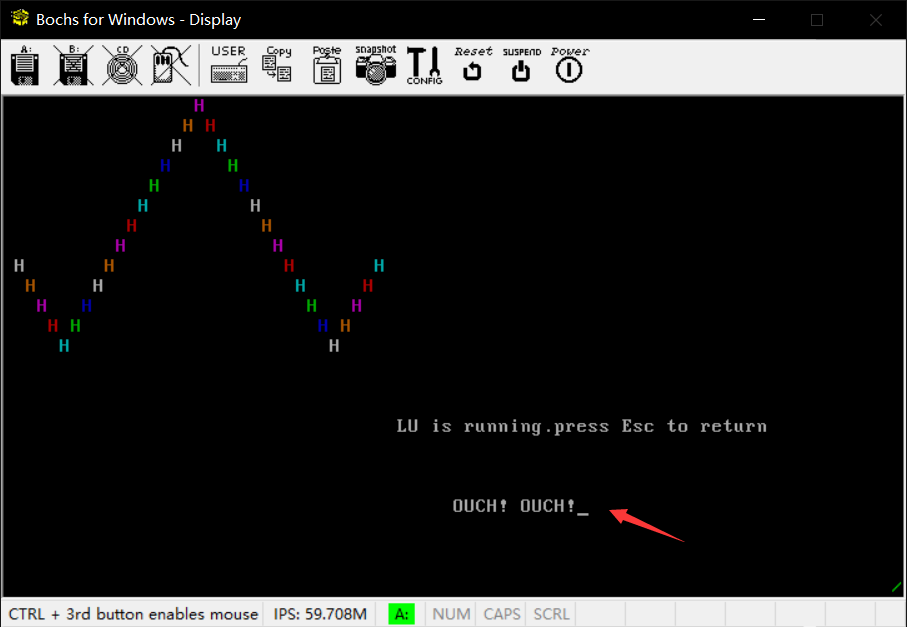
\includegraphics[width=0.8\linewidth]{ouch.png}
  \caption{按下任意键后的"Ouch!Ouch!"}
  \label{fig:timeDisp}
\end{figure}

由于时间中断的效果在虚拟机中观察比比较图片的效果更好,并且虚拟机的时间流逝速度和实际时间不同,可能会看到时间变换较快,因此具体的演示过程可以查看已录制好的OSdemo.mkv

\section{总结与讨论}

% 特色、问题、教训、改进、收获


\subsection{特色,不足与改进}

本程序在上次提供的简洁的shell的基础上增加了实时时间显示。使用gcc+nasm+ld+makefile完成镜像生成的全部步骤。
不足之处是由于键盘按下和放开共触发两次中断,用户会观察到闪烁两次的现象,我没有解决这个问题。

\subsection{收获}

本次实验中,我更加了解了如何利用中断向量表完成自己需要的功能,在丰富shell功能的过程中,我也练习了字符串基本操作函数的编写,在中断程序中使用c函数,在c函数中调用汇编的读端口过程使得
我对混合编程的编程约定也更加熟悉。由于是第二次使用makefile,在编写上更加熟悉了\cite{makefile}。同时,在本报告的编写过程中,我也练习了利用 \LaTeX 编写文档的能力。\cite{lamport94, cite}

\subsection{遇到的问题和感想}
本次实验代码量较小,但是调试的难度与以前相比更大,因为bochs并不会在中断时停下,而我没有很方便的方法能在内存中找到中断程序的代码并设置断点,因此要么只能靠打印数据来调试,
要么把程序移出中断程序来单独调试,比较复杂。在使用BIOS中断获得日期信息时,由于使用了混合编程,按照\_cdecl约定,无论什么类型只要在4个字节内,都是压栈4个字节。因此取出数据时要非常小心。
在调试这段程序时,由于无法找到中断程序的位置,我不得不重新编写单独的程序来调试。
\paragraph{}
使用了离开程序的中断后,我发现用户com程序一旦触发键盘中断bochs就会出现int13_diskette: unsupported AH=10,之后再也无法响应键盘,去掉ouch程序后正常,我认为是嵌套中断导致的问题。
\paragraph{}
在实验开始时,我是直接将中断程序移到内核里去的,当我写了独立的引导程序来执行中断程序后,我发现中断不触发了,是因为没有用sti开中断。并且查阅资料后我才知道中断程序中需要先开中断,
在离开前关中断,否则可能在重要的位置被中断打断出现异常。这说明即使程序运行正常,未必就没有问题。
\paragraph{}
times指令也在我的编程过程中导致了很多问题,由于我习惯将扇区剩余的位置清零,会在代码的最后一段放times指令,结果在放入中断程序时因为失误放在了times的后面,导致中断程序超出了用户程序的2个扇区的大小,
被截断后放入了内存,导致中断处理时的莫名其妙的错误。
\paragraph{}
这次实验中我还找到了之前设计用户程序的bug,如下图,我将控制恢复颜色的语句放在了回到循环开始的语句块之前,导致回到循环之前都会修改字符的颜色值,
由于这个bug被触发是在键盘中断触发时才遇到,因此我一直认为是这次实验中处理中断向量表后导致的错误,花费大量时间在调试上,可见每次实验都必须完全搞清楚才能更轻松的进行下一次实验。
\paragraph{}
在大量的调试过程中,我发现中断程序返回(iret)后,并非直接回到原来的指令处,而是转去执行0xfe830处的代码,这里应该属于bios的,问了其他同学后他们也看到了这个现象。目前并不知道原因,
我也没有找到任何资料说明iret后不会返回,我猜测是bios为中断设计了中断后处理程序。与写保护模式的同学交流后得知,保护模式在iret后是直接返回的。因此大概是bios设计好的工作。

\begin{figure}[H]
  \centering
  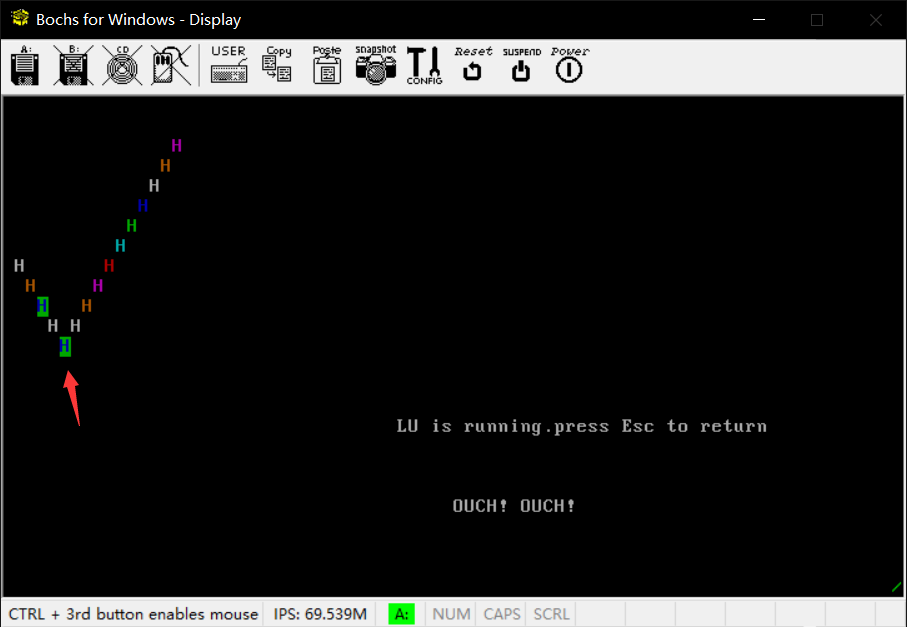
\includegraphics[width=0.8\linewidth]{olduserbug.png}
  \caption{旧用户程序的bug:按下键盘后显示的字符会变色}
  \label{fig:olduserbug}
\end{figure}

\begin{thebibliography}{99}
  
	\bibitem{lamport94}
  Leslie Lamport,
  \textit{\LaTeX: a document preparation system},
  Addison Wesley, Massachusetts,
  2nd edition,
  1994.
  \bibitem{cite}
  Contributors to Wikibooks,
  \textit{LaTeX Bibliography Management.}
  Wikibooks,
  2019., \\
  en.wikibooks.org/wiki/LaTeX/Bibliography\_Management.
  \bibitem{intprocess}
  中断及中断处理过程
  jdksummer,
  2012., \\
  https://www.cnblogs.com/jdksummer/articles/2687265.html
  \bibitem{ostextbook}
  Operating Systems: Internals and Design Principles (8th Edition)
  William Stallings,
  Pearson,
  2014., \\
  \bibitem{makefile}
  how-to-write-makefile,
  \textit{跟我一起写Makefile}
  陈皓,
  2020., \\
 
\end{thebibliography}

\section{附录}

\begin{lstlisting}[language={c},label=utilsForDisp,caption=加工和显示日期时间]
char *strcat(char *dest, const char *src)
{
    char *tmp = dest;

    while (*dest)
        dest++;
    while ((*dest++ = *src++) != '\0');
    return tmp;
}
void strAppend(char*str, char c){
  int len = strlen(str);
  str[len] = c;
  str[len + 1] = '\0';
}
uint8_t bcd2dec(uint8_t bcd)
{
    return ((bcd & 0xF0) >> 4) * 10 + (bcd & 0x0F);
}
\end{lstlisting}

%----------------------------------------------------------------------------------------

\end{document}